\documentclass[handout,fleqn, t]{beamer}

\usepackage{multirow}

\usepackage{tikz}
\usetikzlibrary{graphs}
\usetikzlibrary{graphdrawing}
\usetikzlibrary{positioning,shapes.geometric}
\usetikzlibrary{arrows.meta}
\usegdlibrary{layered,force}

\usepackage{caption}
\captionsetup[figure]{name=}

\usepackage{pgfpages}
\pgfpagesuselayout{2 on 1}[letterpaper,border shrink=5mm]
\pgfpageslogicalpageoptions{1}{border code=\pgfusepath{stroke}}
\pgfpageslogicalpageoptions{2}{border code=\pgfusepath{stroke}}
\pgfpageslogicalpageoptions{3}{border code=\pgfusepath{stroke}}
\pgfpageslogicalpageoptions{4}{border code=\pgfusepath{stroke}}

\title{Graph Theory}
\subtitle{GBW ACSL - Contest \#3}
\author{Clayton O'Neill --- clayton@oneill.net}
\date{2015-2016}

\setbeamertemplate{footline}[frame number]

\begin{document}

\frame{\titlepage}

\frame {
  \frametitle{What is Graph Theory?}
    Graph theory deals with problems that are described in terms of points and
    the connections between the.  Examples include friend relationships in
    social media, an airline route map or a flow chart.  A graph is a
    mathematical way of modeling these sort of situations.
   
  \vspace{1em}
  A graph has two key parts:
  \begin{itemize}
    \item Vertices (also known as nodes)
    \item Edges (also known as connections)
  \end{itemize}
}

\frame {
  \frametitle{What Does a Graph Look Like?}

  The graphs below show examples of the two major types of graphs.  In
  \underline{undirected} graphs the edges simply show what vertices (or nodes)
  are connected.  In \underline{directed} graphs the edges also have a
  direction.  If two nodes are connected in both directions then the arrow will
  be shown at both ends of the edge.  In ACSL we will deal mostly with directed
  graphs.  What are some examples of directed and undirected graphs you can
  think of?

  \begin{columns}
    \begin{column}{0.5\textwidth}
      \begin{figure}
        \tikz [>=Stealth]
        \graph [spring layout, nodes=draw] {
          A--B;
          B--C;
          C--D;
          D--B;
          D--E;
        };
        \caption{Undirected Graph}
      \end{figure}
    \end{column}
    \begin{column}{0.5\textwidth}
      \begin{figure}
        \tikz [>=Stealth]
        \graph [spring layout, nodes=draw] {
          A->B;
          B->A;
          B->C;
          C->D;
          D->C;
          D->B;
          D->E;
        };
        \caption{Directed Graph}
      \end{figure}
    \end{column}
  \end{columns}
}

\frame {
  \frametitle{Graph Notation}
  In the graph below, it has the follow nodes or vertices: A, B, C, D and E.
  
  \vspace{1em}
  The edges (or connections) would be: AB, BA, BC, CD, DC, DB and DE.  The
  edges are specified by listing first the vertex that the connection is from,
  and then the vertex that the connection is to.  Note that listing AB and BA
  means that there is a bidirectional edge between those nodes.  Listing CD and
  DC also gives us a bidirectional edge
  
  \begin{figure}

  \tikz [>=Stealth]
  \graph [spring layout, nodes=draw] {
    A->B;
    B->A;
    B->C;
    C->D;
    D->C;
    D->B;
    D->E;
  };
  \end{figure}
}

\frame {
  \frametitle{Graph Vocabulary I}
  \begin{itemize}
    \item A \textit{path} between two vertices is a list of vertices that would
      be traveled through.  In the previous graph, \textit{ABCDE} is a path
      from A to E.

    \item A \textit{simple path} is a path that does not visit a vertex more
      than once.  \textit{ABCDE} is a simple path, but \textit{ABCDCDE} is not.

    \item A \textit{cycle} is a path that begins and ends at the same vertex.
      For example: \textit{ABCDBA}.  Since a cycle is a circle, you can rotate
      it and describe the same cycle.  For example: \textit{ABCDBA} is the same
      as \textit{BCDBAB}.

    \item A \textit{tree} is a graph that has no cycles.

    \item A \textit{directed acyclic graph} or \textit{DAG} is a directed graph
      that has no cycles.

    \item A directed graph is also known as a \textit{digraph}.
  \end{itemize}
}

\frame[plain] {
  \begin{figure}
    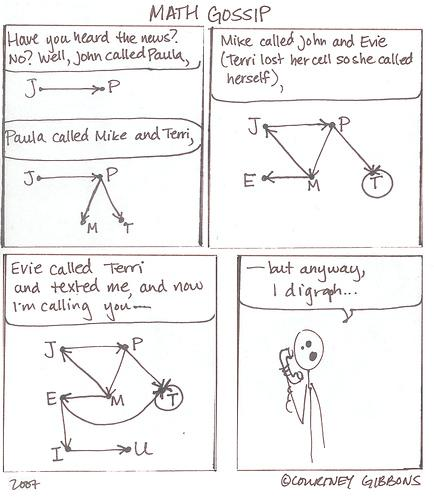
\includegraphics[width=0.70\linewidth]{2007-04-06-mathgossip.jpg}
  \end{figure}
}

\frame {
  \frametitle{Graph Vocabulary II}
  \begin{itemize}
    \item A \textit{connected} graph is one where there is a path from any
      vertex to any other vertex.

    \item A graph that is not \textit{connected} is made up of
      \textit{connected components}.  The graph on the right is made up of two
      connected components: \textit{\{A, B, C, D\}} and \textit{\{E, F \}}.
  \end{itemize}

  \begin{columns}
    \begin{column}{0.5\textwidth}
      \begin{figure}
        \tikz [>=Stealth]
        \graph [spring layout, nodes=draw] {
          A--B;
          A--E;
          B--C;
          B--F;
          C--D;
          D--B;
          E--F;
        };
        \caption{Connected Graph}
      \end{figure}
    \end{column}    \begin{column}{0.5\textwidth}
      \begin{figure}
        \tikz [>=Stealth]
        \graph [spring layout, nodes=draw] {
          A--B;
          B--C;
          C--D;
          D--B;
          E--F;
        };
        \caption{Unconnected Graph}
      \end{figure}
    \end{column}
  \end{columns}
}

\frame {
  \frametitle{Adjacency Matrix}

  There are two primary ways to describe a graph.  You can list all of the
  vertices and edges, or you can use a \textit{matrix} or array to describe
  them.  When using a matrix, the table will be square, with a height and width
  equal to the number of vertices.  The vertical axis shows where the edge
  starts and the horizontal axis shows where the edge ends.

  \vspace{1em}
  \begin{columns}
    \begin{column}{0.5\textwidth}
      \begin{center}
        \begin{tabular}{c c | c c c c}
          {} & {} & \multicolumn{4}{c}{\small{to}} \\
          {} & {} & A & B & C & D \\
          \hline
          \parbox[t]{1mm}{\multirow{4}{*}{\rotatebox[origin=c]{90}{\small{from}}}}
          {} & A & 0 & 1 & 0 & 0 \\
          {} & B & 1 & 1 & 1 & 1 \\
          {} & C & 0 & 0 & 1 & 1 \\
          {} & D & 1 & 1 & 0 & 1 
        \end{tabular}
      \end{center}
    \end{column}    \begin{column}{0.5\textwidth}
      \begin{figure}
        \tikz [>=Stealth]
        \graph [spring layout, nodes=draw] {
          A->B;
          A->B;
          B->[loop below] B;
          B->A;
          B->C;
          C->[loop below] C;
          C->D;
          D->B;
          B->D;
          D->A;
        };
      \end{figure}
    \end{column}
  \end{columns}
}

\frame {
  \frametitle{Graph Vocabulary III}
  \begin{itemize}
    \item A \textit{complete} graph is one where the adjacency matrix is
      \textbf{all} ones.

    \item A \textit{dense} graph is one where the adjacency matrix is
      \textbf{mostly} ones.

    \item A \textit{sparse} graph is one where the adjacency matrix is
      \textbf{mostly} zeros.
  \end{itemize}
  \begin{center}
    \begin{tabular}{c c | c c c c}
      {} & {} & \multicolumn{4}{c}{\small{to}} \\
      {} & {} & A & B & C & D \\
      \hline
      \parbox[t]{1mm}{\multirow{4}{*}{\rotatebox[origin=c]{90}{\small{from}}}}
      {} & A & 0 & 1 & 0 & 0 \\
      {} & B & 1 & 1 & 1 & 1 \\
      {} & C & 0 & 0 & 1 & 1 \\
      {} & D & 1 & 1 & 0 & 1 
    \end{tabular}
  \end{center}
}

\frame {
  \frametitle {What Do You Need to Know?}
  \begin{enumerate}
    \item How to draw a graph from a list of edges.
    \item How to draw a graph from an adjacency matrix.
    \item How to draw a an adjacency matrix from a graph drawing.
    \item How to find paths of a given length from a vertex.
  \end{enumerate}
  
  Items 1, 2 and 3 are fairly straightforward and just require some practice
  and understanding how adjacency matrices work.  For item 4 there are two
  primary techniques.
}

\frame {
  \frametitle{Finding the Number of Paths from a Vertex: Inspection}
  
  The first method for finding paths is "by inspection".  If you were asked to
  find all paths of length two in the graph below, you would start at each node
  and traverse the graph mentally to find all of the options.  You would find
  that the only length two paths were AAC, CAA, BBC and BCA.  This approach is
  the simplest and works well on smaller sparser graphs. On larger denser
  graphs it can get confusing.
  
  \begin{figure}
    \tikz [>=Stealth]
    \graph [layered layout, nodes=draw] {
      C->A;
      A->[loop left]A;
      A->C;
      B->C;
      B->[loop right]B;
      { [same layer] A, B };
    };
  \end{figure}

}

\frame {
  \frametitle{Finding the Number of Paths: Matrix Multiplication I}
  
  With \textit{matrix multiplication} you can find all paths of a specific
  length in a single operation, but it is more complicated.  The first step in
  this technique is to produce an adjacency matrix for the graph:
  
  \begin{columns}
    \begin{column}{0.5\textwidth}
      \begin{figure}
        \tikz [>=Stealth]
        \graph [layered layout, nodes=draw] {
          C->A;
          A->[loop left]A;
          A->C;
          B->C;
          B->[loop right]B;
          { [same layer] A, B };
        };
      \end{figure}
    \end{column}
    \begin{column}{0.5\textwidth}
      \begin{center}
        \begin{tabular}{c | c c c}
          {} & A & B & C \\
          \hline
          A & 1 & 0 & 1 \\
          B & 0 & 1 & 1 \\
          C & 1 & 0 & 0 
        \end{tabular}
      \end{center}
    \end{column}
  \end{columns}
  \vspace{2em}

  Note: In most ACSL materials you will not see the vertex names on the
  adjacency matrix.  It is shown here only to clarify.
}

\frame {
  \frametitle{Finding the Number of Paths: Matrix Multiplication II}
  \begin{itemize}
    \item The adjacency matrix shows how many paths there are between two
      vertices of length 1.  

    \item If you multiply the matrix times itself, or square it,  you will get
      the number of paths between two vertices of length 2.

    \item You can continue this pattern, raising the adjacency matrix to any
      point to find out how many paths of that length.

    \item For example: a matrix multiplied by itself 3 times (or cubed) will
      show all paths of length 3 in the graph.  Multiplying it by itself 4
      times will return all paths of length 4 in the graph, and so on.
  \end{itemize}
}

\frame {
  \frametitle{Finding the Number of Paths: Matrix Multiplication III}
  
  How do we multiply a matrix by itself?  Assume we have the 3x3 matrix shown
  below.  To derive the answer for each cell in the resulting matrix, we have
  to multiply the rows and columns and then add the results:

  \[
      \begin{vmatrix}
        A & B & C \\
        D & E & F \\
        G & H & I 
      \end{vmatrix}
      x
      \begin{vmatrix}
        A & B & C \\
        D & E & F \\
        G & H & I 
      \end{vmatrix}
      =
  \]
  \[
      \begin{vmatrix}
        (AA+DB+CG) & (AB+BE+CH) & (AC+BF+CI) \\
        (AD+DE+GF) & (BD+EE+FH) & (DC+EF+FI) \\
        (AG+DH+GI) & (GB+HE+IH) & (GC+HF+II) 
      \end{vmatrix}
  \]

  As you can see, this requires a large amount of arithmetic.  When doing the
  square of the matrix this isn't too bad, since all the numbers you're working
  with are zero or one.
}

\frame {
  \frametitle{Finding the Number of Paths: Matrix Multiplication IV}
  
  Below is shown the adjacency matrix for the graph shown earlier and the
  result of squaring it.
  
  \begin{figure}
  \[
    \begin{vmatrix}
      1 & 0 & 1 \\
      0 & 1 & 1 \\
      1 & 0 & 0
    \end{vmatrix}^2 =
    \begin{tabular}{ c | c c c }
      {} & A & B & C \\
      \hline{}
      A & 2 & 0 & 1 \\
      B & 1 & 1 & 1 \\
      C & 1 & 0 & 1 
    \end{tabular}
  \]
  \end{figure}
  
  Because we raised the adjacency matrix to the second power, each entry in the
  matrix indicates how many length two paths there are from the \textit{x} and
  \textit{y} axes.  For example, A/A indicates there are two length two paths
  from the vertex A back to itself.  There are zero length two paths from A to
  B, and one length two path from vertex A to C.
}

\end{document}
